\documentclass[a4paper,11pt]{article}
\usepackage{t1enc}
\usepackage[space]{grffile}
\usepackage[round, longnamesfirst]{natbib}  % Bindet den natbib-standard fuer das Zitieren ein
\usepackage{epsfig}
\usepackage{chngcntr}
\usepackage[latin1]{inputenc}   % Ermoeglicht Sonderzeichen direkt einzugeben
\usepackage[T1]{fontenc}        % Garantiert saubere Worttrennung bei Umlauten etc.
\usepackage{color}              % Farbpaket
\usepackage{amsmath,amsfonts,amssymb}   % ermoeglicht mathematische Sonderzeichen
\usepackage[english]{babel}     %
\usepackage{ae}                 %
\usepackage{graphicx}
\usepackage{longtable}          % zum erstellen von Tabellen ber mehrere Seiten
\usepackage{multirow}           % zum Verbinden von Zeilen innerhalb einer Tabelle
%\usepackage{pictexwd}           % PicTex, ein Graphikpaket
\usepackage{pst-all, multido}   % psTricks, ein Graphikpaket
\usepackage{url}
\usepackage[doublespacing]{setspace}
\usepackage{booktabs,caption,fixltx2e,array,dcolumn}
\usepackage{parskip}
\usepackage{etoolbox}
\usepackage{tabularx}
\usepackage{caption}
\usepackage{subcaption}
%\usepackage{morefloats}
\usepackage[section]{placeins} % Mit FloatBarrier kann verhindert werden, dass Float in der nächsten Section angezeigt werden
\usepackage[bottom]{footmisc} % Fußnoten werden ganz unten angezeigt
\setcitestyle{authoryear, open={((},close={))}}

\newcolumntype{L}[1]{>{\raggedright\arraybackslash}p{#1}} % linksbündig mit Breitenangabe
\newcolumntype{C}[1]{>{\centering\arraybackslash}p{#1}} % zentriert mit Breitenangabe
\newcolumntype{R}[1]{>{\raggedleft\arraybackslash}p{#1}} % rechtsbündig mit Breitenangabe

\makeatletter
\interfootnotelinepenalty 10000
\patchcmd{\Ginclude@eps}{"#1"}{#1}{}{}
\makeatother

\makeatletter
\newcommand\tageq{%
  \ifmeasuring@\else
    \refstepcounter{equation}%
  \fi
  \tag{\theequation}%
}
\makeatother

\newcommand\fnote[1]{\captionsetup{font=tiny}\caption*{#1}}

%\parindent 0cm
%\renewcommand{\baselinestretch}{1}

\renewcommand{\bibnumfmt}[1]{#1.}
\bibpunct{(}{)}{;}{a}{,}{,}

%%%%%%%%%%%%%%%%%%%%%%%%%%%%%%%%%%%%%%%%%%%%%%%%%%%%%%%%%%%%%%%%%%%%%%%%%%%%%%%%%%%%%%%%%%%%%%%%%%%%%%%%%%%%%%%%%%%%%%%%%%%%%%%%%%%%


% ________________ EINRICHTEN DES DOKUMENTS ______________________%

%\bibliographystyle{plainnat}    % legt den Stil fuer das Inhaltsverzeichnis fest

\oddsidemargin 0.0in \evensidemargin 0.0in \textwidth 15.5cm \topmargin -0.8in \textheight 24.5cm
\setlength{\parskip}{1pt}
\setlength{\parindent}{0pt}
\renewcommand{\baselinestretch}{1}


\setlength{\intextsep}{0.5cm} % Legt den Abstand zwischen Gleitobjekten und dem darüber und darunter angeordneten Fließtext fest.

%\oddsidemargin 0.1in \evensidemargin 0.1in \textwidth 15.5cm \topmargin -0.4in \textheight 24.5cm
%\parindent 0cm      % legt die Seitenraender fest

\pagestyle{plain}          % leere Kopfzeile, Seitennummer in der Mitte der Fusszeile

\newcommand{\bs}{\boldsymbol}  % shortcut zur Erzeugung von fetten Sympolen in der Mathe-Umgebung

%\renewcommand{\baselinestretch}{1.25}
% 1,5 -facher Zeilenabstand (Standard ist 1,2-facher Zeilenabstand, also 1,2*1,25 = 1,5

\begin{document}

\pagenumbering{roman}   % roemische Zahlen zur Seitennumerierung


%%%%%%%%%%%%%%%%%%%%%%%%%%%%%%%%%%%%%%%%%%%%%%%%%%%%%%%%%%%%%%%%%%%%%%%%%%%%%%%%%%%%%%%%%%%%%%%%%%%%%%%%%%%%%%%%%%%%%%%%%%%%%%%%%%%%%%%5


\begin{titlepage}       % Umgebung fuer Titelseite, frei gestaltbar

\thispagestyle{empty}   % keine Numerierung auf Titelseite

\begin{center}

\includegraphics[width=13cm]{Bild.png}
\end{center}

\begin{center}

\vspace*{1.5cm}
{\bf  \Large Assignment \#5: Monte Carlo Methods - Improving Accuracy and Efficiency} \\
\vspace*{2cm} 
\textbf{B473 Numerical Methods in Finance}
\\
Prof. Dr.-Ing. Rainer Sch\"obel
\\
\vspace*{0.5cm} 
Winter Term 2016-2017\\
\end{center}

\vfill
\begin{flushright}
    \emph{Konstantin Smirnov}\\
    \textit{Student-ID: 3980253}\\
     \textit{ Economics and Finance}\\
 T\"ubingen, \today
  




\end{flushright}



% 
% \begin{center}
% $ $			% oeffnet und schliesst eine Matheumgebung (Trick, um den Titel nach unten zu rutschen
% \vspace{4cm}
% 
% {\LARGE TITEL}
% \vskip 4cm
% 
% Diese Seite ist frei gestaltbar
% \end{center}

\end{titlepage}

\newpage                % erzwingt an dieser Stelle einen Seitenumbruch

\listoffigures
\newpage


\tableofcontents

\newpage
\pagenumbering{arabic}      % Seitenzahlen wieder arabisch numerieren
\setcounter{page}{1}        % Ruecksetzen des Seitenzahlzaehlers auf 1
\section{Introduction}
This assignment discusses another famous and important tool of computational finance, the Monte-Carlo approach. Due to its simplicity and flexibility it is widely used in practice to solve numerical issues. In this assignment, the different Monte Carlo techniques will be applied on option pricing theory. 

As we know, in option-pricing it is required to compute the risk-neutral probability of an underlying, with respect to the stoachstic differential equation (SDE), which can alternatively expressed as an integral I. Generally speaking, in a stochastic framework, this can also be expressed as the expected value $\mathbf{E}$[g(U)]. In a simple case where the random variable $U \sim (0,1)$ is uniformally distributed, we get following expression (Brandimarte, 2006, p. 221):
\begin{equation*}
I=\mathbf{E}[g(U)] = \int_0^1 g(x)d(x)
\end{equation*}
The expected value can be estimated by simply computing the sample mean:
\begin{equation*}
\hat{I}_m = \dfrac{1}{m}\sum^m_{i=1}g(U_i)
\end{equation*}
Under the Law of Large Numbers (LLN) this leads, with a probability of 1, to the population mean I:
\begin{equation*}
\lim_{m\rightarrow\infty} \hat{I}_m = I
\end{equation*} 

To get a more informal idea, Glasserman (2003, p. 30) simplified the methodology of the risk-neutral derivative pricing framework in the following way (''Monte Carlo Recipe for Cookbook Pricing''):\\
\begin{itemize}
\item replace the drift $\eta$ of your SDE with the risk-free interest rate and simulate paths
\item calculate payoff of derivative security on each path
\item discount payoffs at the risk-free rate
\item calculate average over paths\\
\end{itemize}

The advantages of a Monte-Carlo approach are its generality and simplicity. It can handle stochastic volatility models (discussed in chapter 3) or complex exotic options in a relative easy fashion.

But there are also difficulties this approach has to face. In general, three major problems do occur:\\

\begin{itemize}
\item generation of (pseudo)-random numbers
\item discretisation error
\item sampling errors\\
\end{itemize}

In this assignment we will focus mainly on \textit{discretisation} and \textit{sampling} erros, which are closely connected to accuracy and efficiency questions (Brandimarte, 2006, p. 429 - 431). \textit{Discretisation errors} arise from the discretisation of the continuous sample path whereas \textit{sampling errors} occur due to a too small number of simulations \textit{N}, closely related to the LLN.

Accuracy can be improved with an increase in the number of time increments \textit{n} or number of simulations run \textit{N} but this would come with an increase in computational effort. This paper discusses how \textit{discretisation errors} can be decreased by using different discretisation techniques. Specifically, it will be discussed how the \textit{Milstein scheme} can reduce discretisation errors. There exist also various techniques to reduce sampling errors. In this assignment the focus lays on the \textit{control variate technique} to reduce the variance of the sample. Besides this we will consider technical implementation in \textit{MATLAB}.

Note that regardless the just listed theoretical approaches to increase accuracy and efficiency, CPU and GPU performance increased heavily in the last century which is another major source of efficiency gain, in general. Betkaoui, Thomas and Luk (2010) discuss this topic from a technical point of view. They compared technical efficiency by running 1,000,000 simulations of an Asian option. It could be shown that the use of new processor technologies lead to a performance improvement of up to 18-times over a multi-threaded software implementation.

\section{Improving strong convergence with the Milstein scheme}
As we just noted, discretisation errors arise from the discretisation of a continuous function. Therefore we will compare the \textit{Euler Scheme} and a refinement, the \textit{Milstein scheme}, with the continuous path of a stock. Specifically, it will be shown how the \textit{Milstein} scheme can reduce the discretisation error significantly.

\subsection{Theoretical Framework}
Since we are interested in the generation of derivatives, the simulation path of the underlying plays a crucial role in computing the final price (Brandimarte, 2006, p. 431).

A general representation of a typical SDE is:
\begin{equation}
dS_t=a(S_t,t)dt + b(S_t,t)dW_t
\label{GB}
\end{equation}
The most simple discretisation approach with respect to (\ref{GB}) is known as the \textit{Euler scheme}: 
\begin{equation}
dS_t=S_{t+\Delta t} - S_t= a(S_t,t)\Delta t +b(S_t,t)\sqrt{\Delta t} \epsilon
\label{eulerG}
\end{equation}
where $\Delta t$ is the discretisation step and $\epsilon \sim \mathbf{N} (0,1)$. 

More specifically, under geometric Brownian Motion the continuous path of an underlying stock S is defined as:
\begin{equation}
dS_t=\eta S_t dt + \sigma S_t dW_t
\label{cont}
\end{equation}
and with the associated Euler scheme with respect to (\ref{eulerG}):
\begin{equation}
S_{t+\Delta t}=(1+ \eta \Delta t) S_t + \sigma S_t \sqrt{\Delta t}\epsilon
\label{euler}
\end{equation}
Representation (\ref{euler}) is a simple and straight-forward representation of the underlying path. Reducing $\Delta t$ would decrease the discretisation error but this also would come with higher computational effort.

Applying Ito's lemma on equation (\ref{cont}) would also lead to another alternative straight-forward representation:
\begin{equation}
S_T= S(t) exp[(\eta - \dfrac{1}{2} \sigma^2)\Delta t+\sigma \epsilon \sqrt{\Delta t}]
\label{theocont}
\end{equation}
but keep in mind that this kind of transformation (\ref{theocont}) is not always applicable, especially for more complex SDE (Brandimarte,2006, p. 433).

One way to reduce computational burden would be the use of a different discretisation scheme. An alternative to the Euler Scheme is the  \textit{Milstein scheme} which is defined as (Glasserman, 2004, p. 343.):
\begin{equation}
\Delta S= a(S,t)\Delta t + b(S,t)\epsilon\sqrt{\Delta t} + \dfrac{1}{2}bb'(\epsilon^2 -1)\Delta t
\label{milsteintheo}
\end{equation}
where \textit{b'(S,t)} is the partial derivative of the constant b with respect to S. 

In our specific case, when b(S,T)=$\eta$S with b'(S,T)=$\eta$, (\ref{milsteintheo}) this leads to:
\begin{equation}
\Delta S = rS \Delta t + \eta S \varepsilon \sqrt{\Delta t} + \frac{1}{2} \eta^2 S(\varepsilon^2 - 1) \Delta t
\label{milstein}
\end{equation}

When it comes to truncation errors, it can be shown that the Euler scheme approximation (\ref{euler}) has an error of order $O(\Delta t)$  for the drift term and $O(\sqrt{\Delta t})$ for the diffusion term. The truncation error of the diffusion term in the Milstein scheme is of order $O(\Delta t)$, which is an improvement compared to the Euler scheme (Glasserman, 2004, p. 340 - 343).
However, this improvement is not generally the case, so the choice of the scheme depends on the model itself. Indeed, if the diffusion coefficient is independent of the state variable b=b(t), one can show that the truncation errors of both schemes are of the same order. In that case, it would make sense to use an one-step simulation if a closed form solution exists. Only if b depends on the state variable b(S,t), as in our case (\ref{milstein}), then the Milstein scheme is truly superior regarding accuracy and efficiency. Alternatively, one could try to use a transformation to make b independent of the state variable.

In the next section we will compare these schemes by application. Note that a further theoretical discussion can be found in Glasserman (2004, p. 344 - 348).
\subsection{Discussion of Results}
To discuss accuracy and efficiency of the Milstein scheme, following parameters were used to simulate the different stock price paths with a continuous function, the Euler scheme and the Milstein scheme:

\begin{table}[!h]
\centering
\caption{Sample parameters of problem 1}
\begin{tabular}{l|l|l}
\textbf{Description} & \textbf{Variable} & \textbf{Value}  \\\hline
 stock price& S  & 100  \\
 Time to maturity& T - t  & 0.5 \\
 risk-free interest rate& r & 0.0953 \\
 volatility& $\eta$ & 0.25\\
 initialization value of the random generator & seed& 7777
\end{tabular}
\end{table}

In figure \ref{plot1} all three simulated paths with respect to equations (\ref{cont}) (continuous), (\ref{euler}) (Euler) and (\ref{milstein}) (Milstein) were simulated with the given parameters. We used a discretisation step size of 1000 steps in this illustration. In the full scale representation, the scheme approximations look already relatively accurate. However, as you can see in the right plot, the Milstein scheme delivers a more accurate version of the continuous path simulation compared to Euler scheme. 

\begin{figure}[!h]
\centering
\begin{subfigure}[c]{0.5\textwidth}
\caption*{full scale}
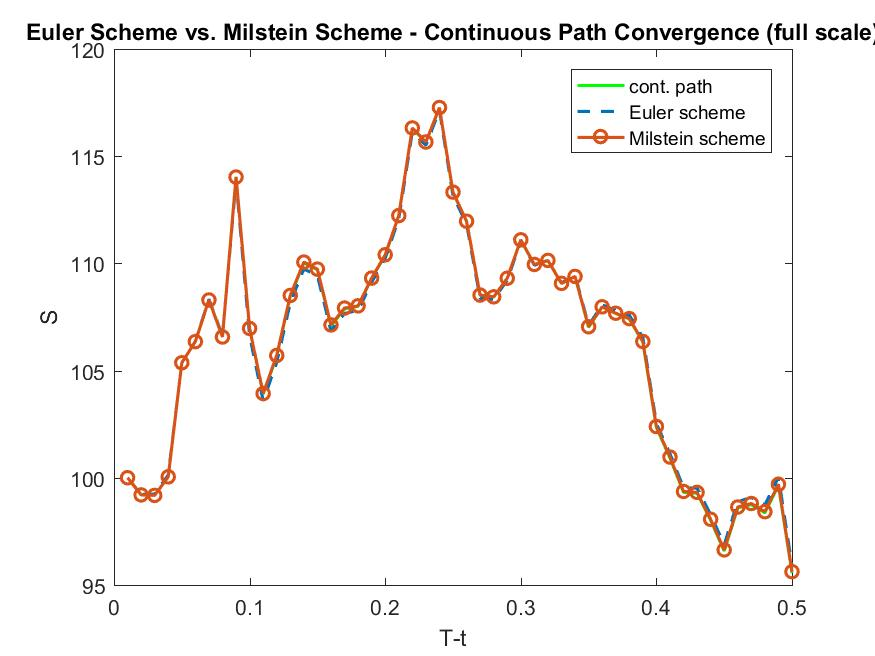
\includegraphics[width=8.5cm]{plot11.jpeg}
\end{subfigure}
\begin{subfigure}[c]{0.4\textwidth}
\caption*{zoomed in}
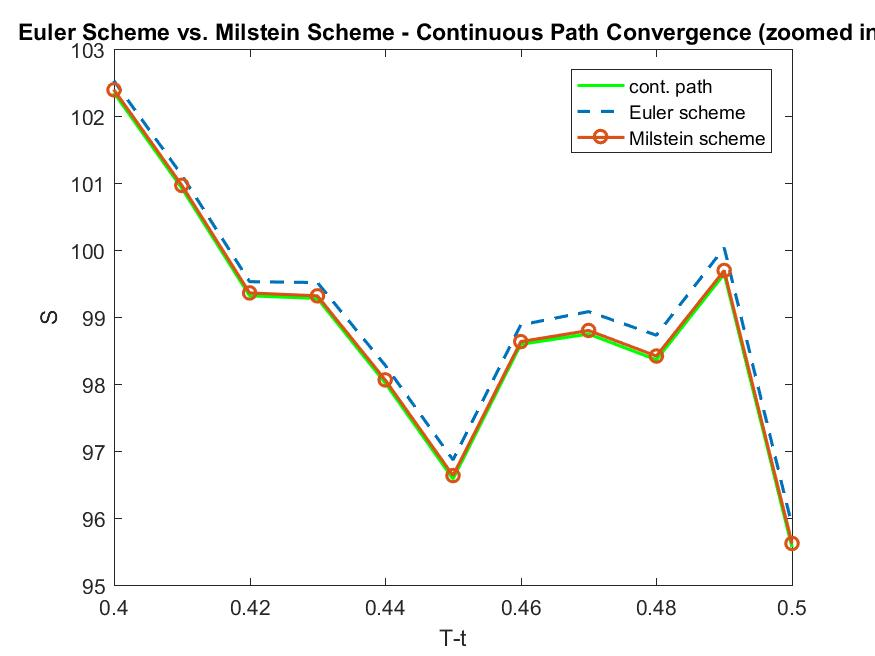
\includegraphics[width=8.5cm]{plot11z.jpeg}
\end{subfigure}
\caption{Euler Scheme vs. Milstein Scheme - Continuous Path Convergence}
\label{plot1}
\end{figure}

To get a better understanding of accuracy and efficiency, the final terminal value of the continuous path is opposed to the terminal values of both schemes for increasing discretisation step size \textit{n} from $1^2$ to $14^{2}$, represented in figure \ref{plot2}. The right figure of this plot additionaly takes account of the discretisation error which is simply the difference between the terminal value and the schemes approximations, respectively for a given \textit{n}.\footnote{This form of step-size increasement was chosen due to graphical illustration.}
\newpage
\begin{figure}[h!]
\centering
\begin{subfigure}[c]{0.5\textwidth}
\subcaption*{Cont. Path Convergence}
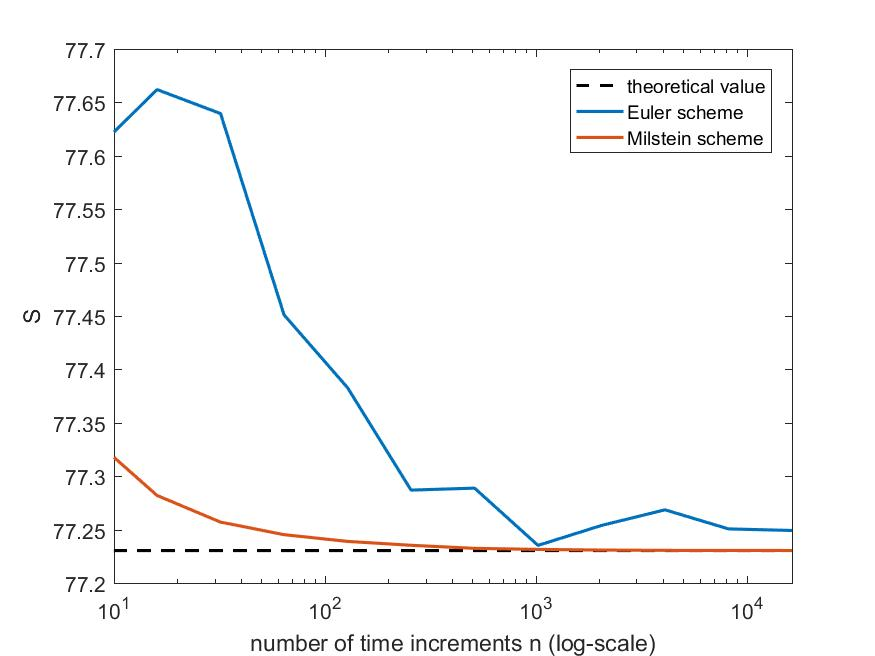
\includegraphics[width=8cm]{plot12.jpeg}
\end{subfigure}
\begin{subfigure}[c]{0.4\textwidth}
\subcaption*{Error Convergence}
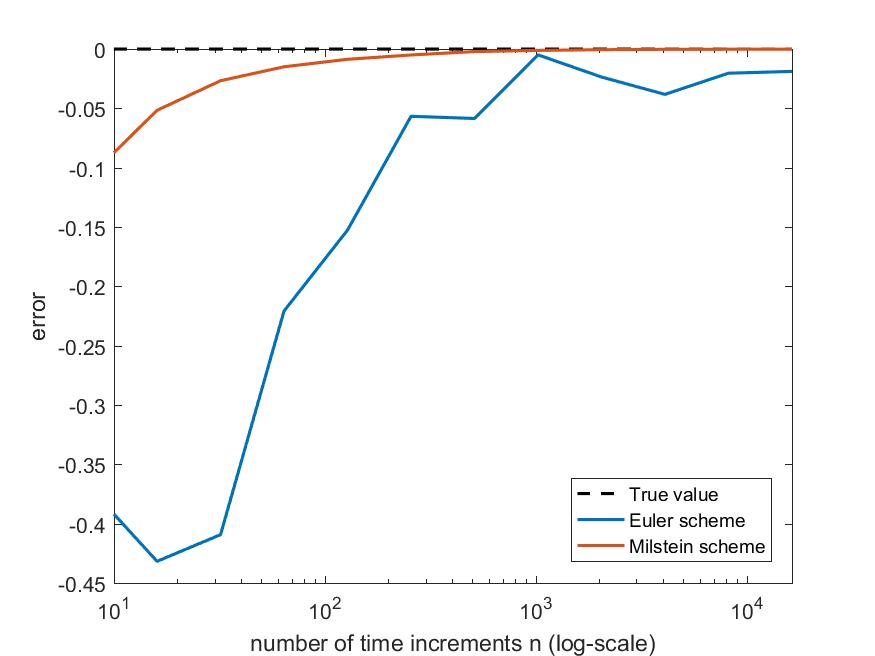
\includegraphics[width=8cm]{plot13.jpeg}
\end{subfigure}
\caption{Euler Scheme vs. Milstein Scheme - Cont. Path Convergence and Discretization Error}
\label{plot2}
\end{figure}

Clearly, in both illustrations, the Milstein scheme delivers more precise results for a small step-size parameter compared to the Euler scheme. With a step-size of n=128 the error of the Milstein schemes has the value of -0.0086 while the error of the Euler scheme still has a relatively big value of -0,1526. With a step-size of n=2048 error of the Milstein scheme is already close to 0 with a value of -0,0005 while the Euler scheme only improved to -0,0234 which is in line with the theory described in the first part of this chapter. Indeed, in our case, the Euler scheme does not directly converge to the true value, even for relatively large discretisation steps leading to systematic errors which makes the Milstein scheme superior when it comes to accuracy.

Note that in this computations for the continuous path, the terminal value of equation (\ref{theocont}) was used which leads to more accurate results compared to continuous path representation (\ref{cont}). In fact, the Milstein scheme does not converge to the terminal value of equation \ref{cont}. This may come from the fact that (\ref{cont}) contains a discretisation error on itself since in practice the function is also discretised.  Hence the more accurate approach (\ref{theocont}) was used, where the Milstein scheme converged to the true value.

\begin{figure}[h!]
\centering
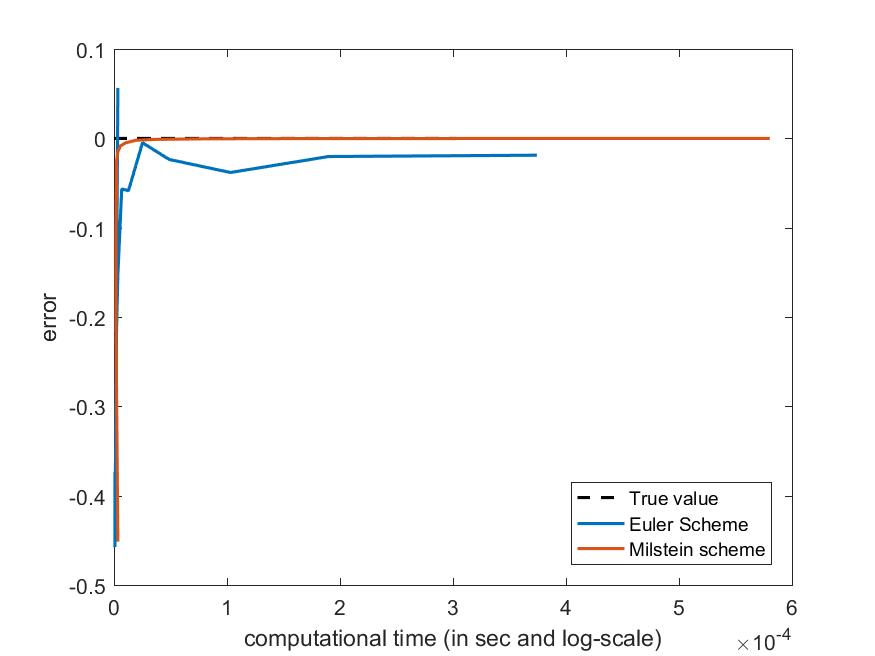
\includegraphics[width=11cm]{plot14.jpeg}
\caption{Euler Scheme vs. Milstein Scheme - Computational Effort}
\label{plot13}
\end{figure}

Since the error of the Milstein scheme vanishes for relative small discretisation steps, generally speaking, it converges faster to the true value but this does not imply that it is the general faster approach. It could be the case that the Milstein algorithm is time costly in its nature. But this can be disproved while having a look on figure (\ref{plot13}). As you can see the Milstein scheme is not only superior when it comes to accuracy but also when it comes to time efficiency in general compared to the Euler scheme. Since, as we just have seen, the accuracy is relatively high, it reaches the true value fast.\footnote{Note that time meisurement highly depends on the hardware and software used for computations.}

Summarized, the Milstein scheme is, in that simple case, superior to the Euler Scheme regarding efficiency and accuracy which is in line with the theory stated in the beginning of the chapter. Keep in mind that these result only holds if the coefficient b depends on the state variable, which is the case in our example.

\subsection{Technical Implementation}
All associated computations of chapter 2 can be called in the main script \textit{problem1.m}. Since we need a stream of pseude-random number stream for the Brownian Motion, the \textit{Rand.Generator} command was used to create a stream of (pseudo)-random numbers with a combined multiple recursive random number generator ('\textit{mrg32k3a}').

The functions \textit{cont.m, euler.m and milstein.m} are called in the main script and basically contain the algorithms with respect to the mentioned equations in the theoretical part of this chapter. 

The given parameters of the assignment and the (pseudo)-random stream, as well as the number of overall increments \textit{nn1} and the discretisation step size \textit{nn2} serve as input parameters. As an output the algorithms deliver the stock price paths as well as terminal values of the stock price path with the given parameters. The \textit{Euler} and \textit{Mils} algorithms additionally output the meisured time of one run.

Since in problem 1 we are interested in the simulated paths in general, the functions were simply called with a \textit{nn11} of 1000 and a \textit{nn12} of 50. 

In the second part of the assignment, the Euler and Milstein algorithms are looped for different squared step sizes \textit{nn22}=$1^2$, $2^2$..., to $14^2$ (due to illustrative reasons) with respect to the input parameters and an overall number of increments \textit{nn21} = 10000. As it was already mentioned,  the analytic solution was used (\textit{SPath}) instead of the disc. continuous version \textit{cont.m}.  All computations can be found in the \textit{accuracy} output matrix where the terminal values and the step-size values are saved. The errors and the time are additionally saved in the \textit{errors\_euler} or \textit{errors\_milstein} and the \textit{time\_efficiency} vectors.

Note here that time measurement is highly subjective since it depends highly on the used hardware and the software of the system. In this assignment, all computations were run on an Windows 10 64-bit operation system with an Intel(R) Core(TM) i7-5500U CPU 2.40 Ghz.

\section{Variance reduction using control variate techniques}
As we described in the beginning of the chapter, inaccuracy in the Monte Carlo approach might arise as a sampling error. In that case, due to the LLN, the variance of the estimate can also be reduced by simply increasing the number of samples N but this would come with an increase in computational time.

In this section we will discuss how the control variate technique (CVT) can increase efficiency by decreasing the relative sampling error without increasing the number of sampled paths. Specifically, we apply this technique on a stochastic volatility derivative model of Sch\"obel and Zhu (1999).

\subsection{Theoretical Framework}
The theoretical framework of the variance reduction technique is described by Glasserman (2003, p. 185 - 186).
Assume there are $Y_1 , Y_2, ...., Y_i$ samples of a discounted payoff of the sampled path. 

If $Y_i$ are identical and independent distributed (i.i.d), the usual estimator of the sample is described as:
\begin{equation}
 \hat{Y}=\mathbb{E}[Y_i]=\frac{1}{n} \sum_{i=1}^n Y_i 
 \label{USUAL}
\end{equation}
which converges under LLN to a probability of 1 with $n \rightarrow \infty$.

Suppose there is another estimate $X_i$ along with $Y_i$ which is also i.i.d. and with the same distribution as $Y_i$ with a known expectation $\hat{X}=\mathbb{E}[X]$. The control variate estimator can then be described, for any fixed b, as:
\begin{equation}
\hat{Y}(b)= \hat{Y} - b(\hat{X} - E[X]) = \frac{1}{n} \sum_{i=1}^n Y_i - b(X_i - \mathbb{E}[X])
\label{CVE}
\end{equation}
where $ \hat{X} -E[X]$ serves as a control in estimating $\mathbb{E}[Y]$.

One can show that the estimator (\ref{CVE}) is unbiased and consistent (with probability 1):
\begin{eqnarray*}
\hat{Y}(b) = \mathbb{E}[Y] \quad and \quad \lim_{n \rightarrow \infty} = \mathbb{E[Y]} 
\end{eqnarray*}
and has a variance of:
\begin{equation*}
Var[Y_i (b)] = \sigma^2_Y - 2b\sigma_X \sigma_Y \rho_{XY} + b^2 \sigma^2 _X = \sigma^2(b)
\end{equation*}
with $\sigma^2_X = Var[X]$, $\sigma^2_Y = Var[Y]$ and with the correlation factor $\rho_{XY}$ between the random variables X and Y.

The estimated variance of the usual estimator is:
\begin{equation}
\hat{\sigma}_{Y}^2 = Var[Y_i]/N;
\end{equation}
and the estimated variance of the CVT is defined as:
\begin{equation}
\hat{\sigma}_{CVT}^2 = Var[Y_i(b)]/N;
\label{sigmaestb}
\end{equation}
If $b^2\sigma_X < 2b\sigma_Y \rho_{XY}$, then the estimated variance of the control variance estimator  $\hat{\sigma}_{CVT}^2 $ is smaller then the estimated variance of the usual estimator   $\hat{\sigma}_{Y}^2$. 

One can show that the optimal b, which minimizes the variance, is:
\begin{equation}
b^* =  \dfrac{\sigma_Y}{\sigma_X} \rho_{XY} = \frac{Cov[X,Y]}{Var[X]}
\label{b}
\end{equation}

In practice, $\mathbb{E}[Y]$ is unknown. Therefore, we use the sample counterparts which are defined as:
\begin{equation}
\hat{b}_N =  \frac{\sum^N_{i=1} (X_i - \hat{X})(Y_i - \hat{Y})}{\sum^N_{i=1} (X_i - \hat{X})^2}
\label{bsample}
\end{equation}

Substituting (\ref{b}) into (\ref{CVE}) results in the variance ratio between the controlled variance estimator and the uncontrolled estimator, which measures the effectiveness of a control variate, we will get:
\begin{equation}
\dfrac{Var[\hat{Y} - b^*(\hat{X} - \mathbb{E}[X])]}{Var[\hat{Y}]} = 1 - \rho^2_{XY}.
\label{efficiency}
\end{equation}
If the algorithms of the usual estimator and the CVT are roughly the same regarding computational time, then the speed up resulting from the control variate can be computed, with respect to equation (\ref{efficiency}), by:
\begin{equation}
\varrho = \dfrac{N}{1 - \rho^2_{XY}} 
\label{efficiency2}
\end{equation}
In other words this expression tells you the number of replications \textit{N} needed with the usual estimate to get the same estimated CVT variance (\ref{sigmaestb}).

Equation (\ref{efficiency}) shows that a high correlation factor would  lead to a sharp increase regarding efficiency. On the other side a relative low correlation factor would only marginally increase efficiency. For example, for N=1, a $\rho$ of = 0.95 would lead to a speed up of around 10x compared to the usual estimator, while an $\rho$ = 0.9 would achieve only half of the speed up of around 5x. Hence a relative high $\rho$ is needed in order to gain efficiency when using this kind of variance reduction technique.

In the following chapter we will apply the usual estimator and the CVT modification on a European call with stochastic volatility (Sch\"obel and Zhu, 1999). The Sch\"obel and Zhu model (SZ-model) is defined as :

\begin{equation}
dS=rSdt + vSdW_1
\label{s}
\end{equation}
where the instantaneous volatility follows a mean-reverting Ornstein-Uhlenbeck process:
\begin{equation}
dv=\kappa(\theta - v)dt + \sigma dW_2
\label{vola}
\end{equation}
where the Brownian motions $dW_1$ and $dW_2$ are correlated: 
\begin{equation*}
\rho dt= dW_1 dW_2
\end{equation*}
with
\begin{equation*}
dW_1=dW_1^*
\end{equation*}
\begin{equation*}
dW_2= \rho dW_1^* + \sqrt{1-\rho^2} dW_2^*
\end{equation*}
\begin{equation*}
dW_1^* dW_2^* = 0
\end{equation*}
where the payoff function of a European Call is defined as:
\begin{equation}
Y_i = e^{-r(T-t)}max(S_{iT}-K,0)
\end{equation}

As a control variate the standard one-dimensional Black-Scholes-Merton (BSM) model is used, which is defined as:
\begin{equation}
dS= rSdt + S \sigma dW_1
\label{BCSM}
\end{equation}
with $dW_1$:
\begin{equation*}
dW_1 = \sqrt{dt} \epsilon
\end{equation*}
The population of mean of $\mathbb{E}$[X] is known since there exists a closed-form solution of the BSM. It is defined as:
\begin{equation}
C_{BCSM}(S,t)=S e^{(h-r)(T-t)}N(d_1)-Xe^{-r(T-t)}N(d_2)
\label{BCSM}
\end{equation}
with
\begin{equation*}
d_1=\frac{ln(\frac{S_t}{X})+(h+0.5\sigma^2)(T-t)}{\sigma \sqrt{T-t}}
\end{equation*}
\begin{equation*}
d_2=d_1-\sigma\sqrt{T-t}
\end{equation*}
where N is normally distributed $N \sim (0,1)$.
\subsection{Discussion of Results}
In the following section following parameters were used for our computations:

\begin{table}[h!]
\centering
\caption{Input parameters for problem 2}
\label{my-label}
\begin{tabular}{l|l|l}
\textbf{Description} & \textbf{Variable} & \textbf{Value}  \\\hline
 stock price& S  & 100  \\
 strike& K  & 100 \\
 Time to maturity& T - t  & 0.5 \\
 risk-free interest rate& r & 0.0953 \\
mean reversion parameter& $\kappa$ & 4.0  \\
 ''volatility of volatility''& $\sigma$ & 0.1 \\
  long-run volatility& $\theta$ & 0.2 \\
   correlation coefficient& $\rho$ & -0.5 \\
   instantaneous volatility of the stock price& v & 0.2 \\
   initialization value of the random generator & seed& 7777
   
\end{tabular}
\end{table}
In the next subsections the effect of an increase in number of samples \textit{N} and in an increase in number of time increments \textit{n} will be analyzed and discussed. 

\subsubsection{Accuracy and Efficiency: the effect of an increase in simulations \textit{N}}

In this examination, the model was discretised with the Euler scheme, where the number of time increments \textit{n} was fixed to n=5000. According to the assignment, the real price of this call is 8.243.

First, the efficiency factor $\varrho$ given in (\ref{efficiency2}) was computed. The variables X and Y of our CVT estimator are highly correlated with $\rho_{XY}$  = 0.9851 (for a N = 10,000) and hence the CVT model should reduce variance significantly. Indeed, our computations proofed this finding. For a N=1000, the $\varrho$ is approximately $\sim$ 30491, so to achieve the same variance as the CVT with N=1000, the usual estimator would need N = 30491 simulations. Hence the CVT in our case is around 30.50x times more accurate then the usual estimator.

To illustrate how accuracy is improving, we additionally compute the $95\%$-confidence intervals (CI) of the estimates. The CVT CI's are defined as (Glasserman, 2003, p. 195):
\begin{equation}
CI_{+/-} = \hat{Y}(b) \pm 1.96 \dfrac{\hat{\sigma}}{\sqrt{N}}
\end{equation}
and for the usual estimator, the 95\% - CIs are defined as:
\begin{equation}
CI_{+/-} = \hat{Y} \pm 1.96 \dfrac{\hat{\sigma}}{\sqrt{N}}
\end{equation}
where $\hat{\sigma}$ is the estimated standard deviation.
\begin{figure}[!h]
\centering
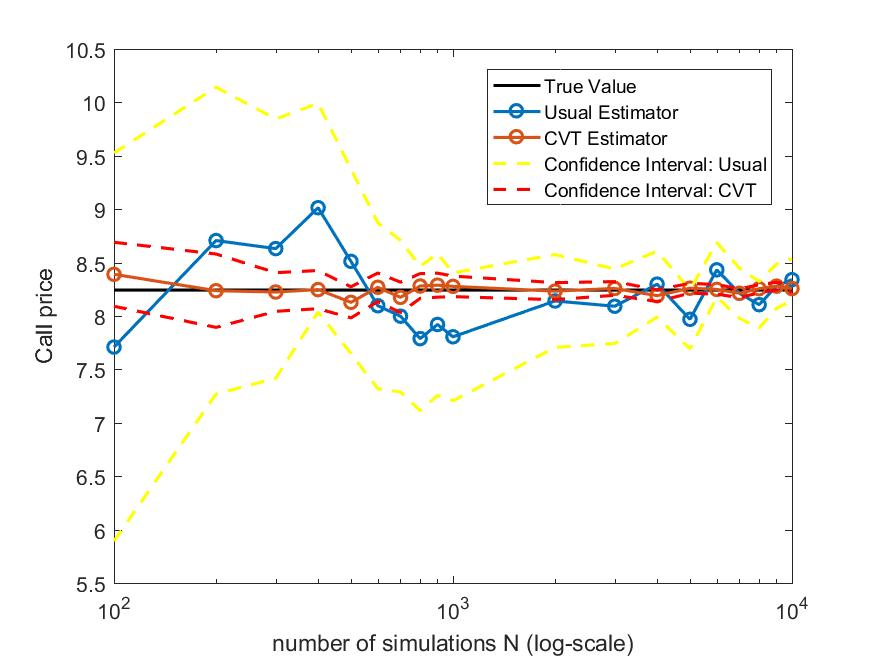
\includegraphics[width=11cm]{plot21.jpeg}
\caption{Accuracy of the CVT for increasing N - Usual Estimator vs. CVT}
\label{plot21}
\end{figure}

Illustration \ref{plot21} shows the convergence behavior of the simulation with of the usual (Euler) estimator and the CVT estimator in an increase in number of simulations \textit{N}, reaching from 100:100:1000 and 1000:1000:10000.{\footnote{This intervals were choosen due to illustrative reasons.}

The findings in these plots are in line with the theory. The CVT estimator already converges smoothly close to true value (8.243) even for relatively small number of simulation paths \textit{N} where as the usual estimator oscillates vigorously, specifically in the beginning, around the true value. The CI's of the CVT are narrow where as the CI's of the usual estimator are relatively bright and only slowly get closer with increasing N. However, for that given intervals, even for large N, the usual estimator is not able to achieve the same accuracy as the improved CVT.

\begin{figure}[!h]
\centering
\begin{subfigure}[c]{0.5\textwidth}
\caption*{Estimation Errors}
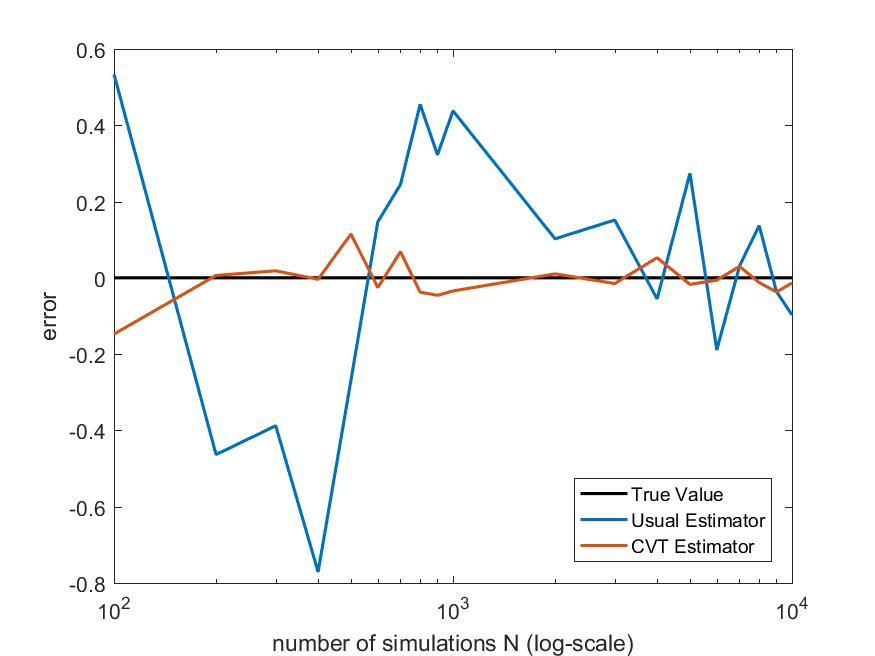
\includegraphics[width=8.5cm]{plot23.jpeg}
\end{subfigure}
\begin{subfigure}[c]{0.4\textwidth}
\caption*{Estimated Standard Deviation}
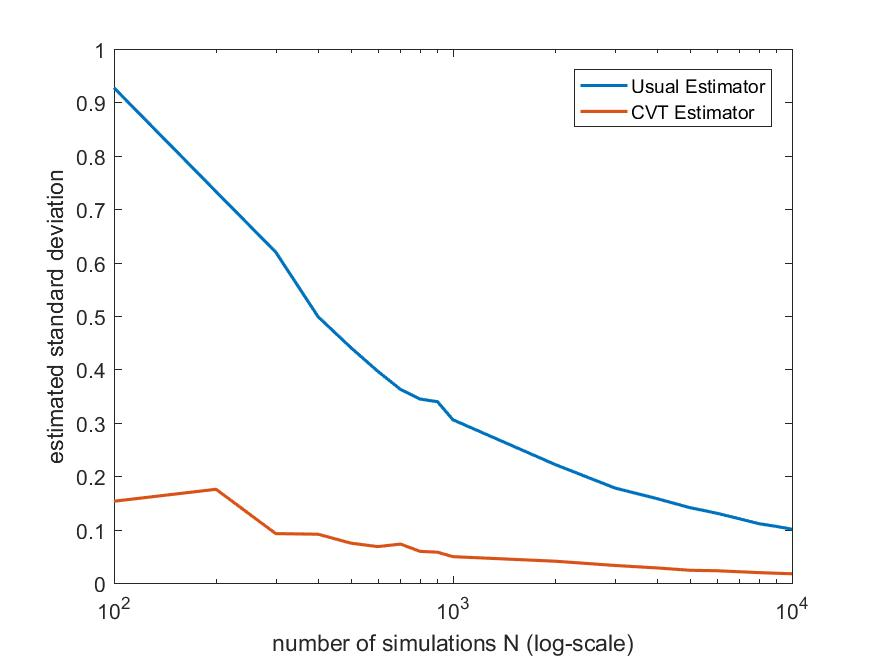
\includegraphics[width=8.5cm]{plot22.jpeg}
\end{subfigure}
\caption{Accuracy of the CVT for increasing N - Estimated Error and  Estimated Standard Deviation}
\label{plot22}
\end{figure}

Figure \ref{plot22} highlights this result. The left figure shows the estimation errors for an increase in sample paths \textit{N} with respect to the true value of 8.243. The estimated error for the CVT converges smoothly to the 0-error line, whereas the usual estimator has high oscillations which weaken only slowly with high N. The right plot shows the estimated standard deviation $\hat{\sigma}_{Y}/\sqrt{N}$ and $\hat{\sigma}_{CVT}/\sqrt{N}$. While for the CVT, the standard deviation starts already with relative small values, the values of the usual estimator starts with a high deviation and only drive slowly towards 0. However, it can never reach the precision of the CVT estimator for that specific \textit{N}. You can also observe the big difference between the two estimated standard deviations, which approves the findings regarding $\varrho$ that the CVT is around 30x more accurate.

\begin{figure}[!h]
\centering
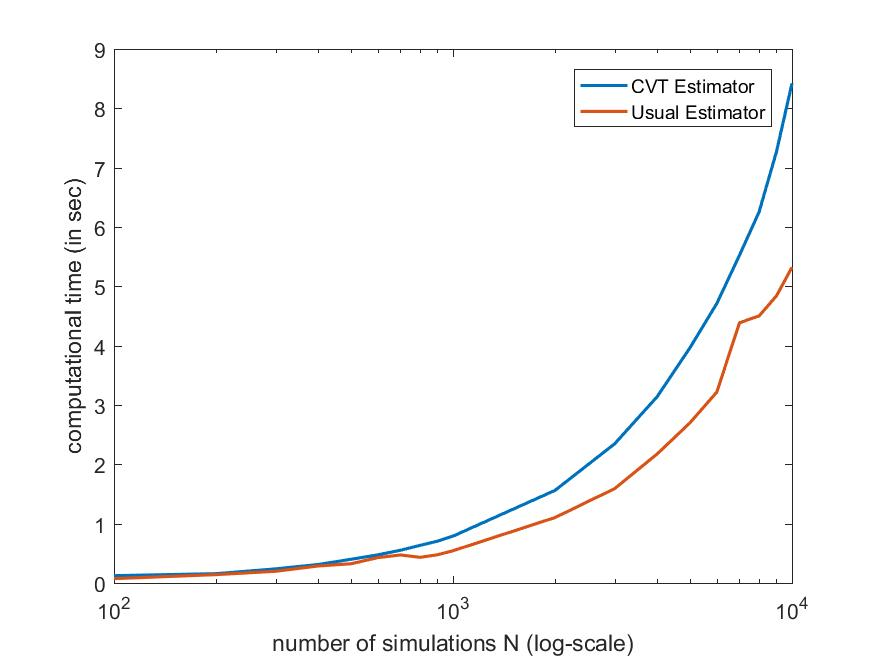
\includegraphics[width=11cm]{plot26.jpeg}
\caption{Efficiency of the CVT for increasing N - absolute Computational Effort}
\label{plot26}
\end{figure}
\newpage
Summing up, the CVT modification,  due to that highly correlated $\rho_{XY}$ in that specific case, is truly superior to the usual estimator. This is also proven graphically. However, from an efficiency point of view, all these findings would not matter if computational burden of the CVT algorithm, f.e. due to too many complex operations, would be too time costly compared to the variance reduction improvement.

Figure \ref{plot26} shows how many seconds the usual estimator or the CVT need to estimate a price for \textit{N} number of generated sample paths. For a small number of observations paths, the time effort is only marginal, while for N=10000, the computation indeed needs 3 seconds longer then the usual estimator. From an absolute point of view, the CVT algorithm is more time costly which is not surprising since by its nature it has to handle more operations then the usual estimator algorithm.

\begin{figure}[!h]
\centering
\begin{subfigure}[c]{0.5\textwidth}
\caption*{Computational Time vs. Price}
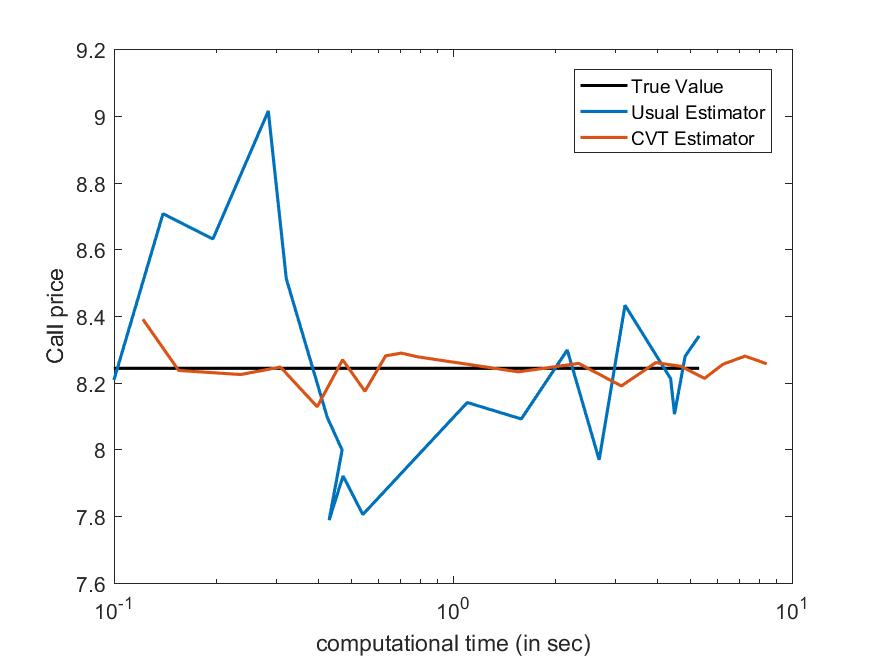
\includegraphics[width=8.5cm]{plot24.jpeg}
\end{subfigure}
\begin{subfigure}[c]{0.4\textwidth}
\caption*{Computational Time vs. $\hat{\sigma}$}
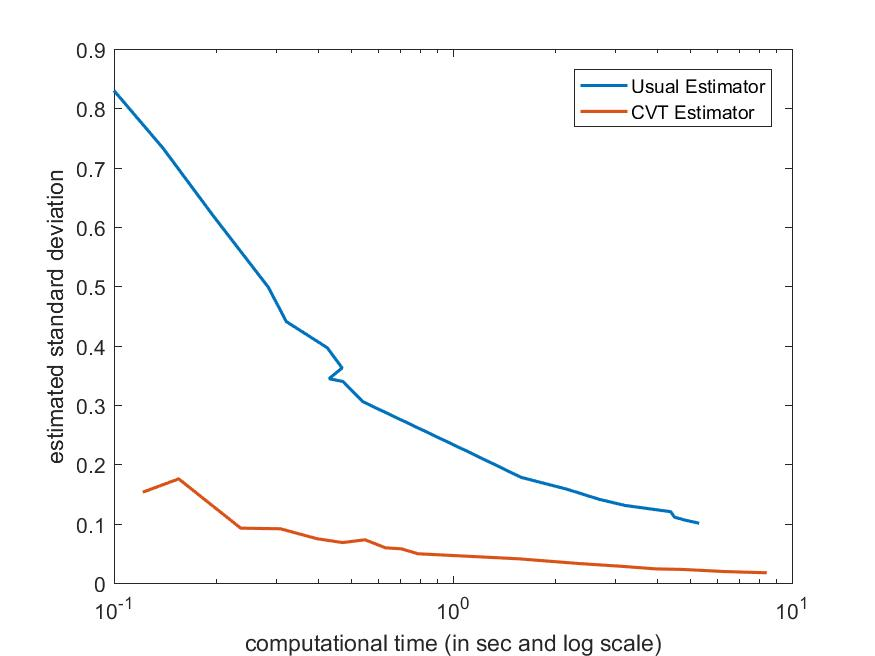
\includegraphics[width=8.5cm]{plot25.jpeg}
\end{subfigure}
\caption{Efficiency of the CVT for increasing N - Price Convergence and  $\hat{\sigma}$}
\label{plot27}
\end{figure}

Nonetheless, in plot \ref{plot27} these findings can be put into perspective. The illustrations show the computational effort  plotted against the Call price and the estimated standard deviation. The left plot again shows the high osciliation of the usual estimator. The computations might be shorter from an absolute point of view, but indeed the usual estimator is not able to deliver precise results as good as with CVT, in that given time. These findings are also  substantiated when observing the measured computational time vs. estimated standard deviation, represeted in the right figure of the plot.

Summing up, the CVT is not only superior from an absolute accuracy point of view, but also superior when it comes to time efficiency.  Keep in mind that the CVT is only efficient if the correlation $\rho_{XY}$ is high enough which might not be the usual case when it comes to practical application.

\subsubsection{Accuracy and Efficiency: the effect of refining the number of time increments \textit{n}}
In the next part of this subchapter, we will briefly discuss the effect of an increase in the number of time increments \textit{n}, as it was discussed in chapter 2, on accuracy and efficiency of the usual estimate and the CVT. The algorithms were run with an increase in \textit{n} from $2^1$, $2^2$ up to $2^{14}$ for a fixed number of simulations \textit{N} = 1000 and N = 10,000.

\begin{figure}[!h]
\centering
\begin{subfigure}[c]{0.5\textwidth}
\caption*{N=1000}
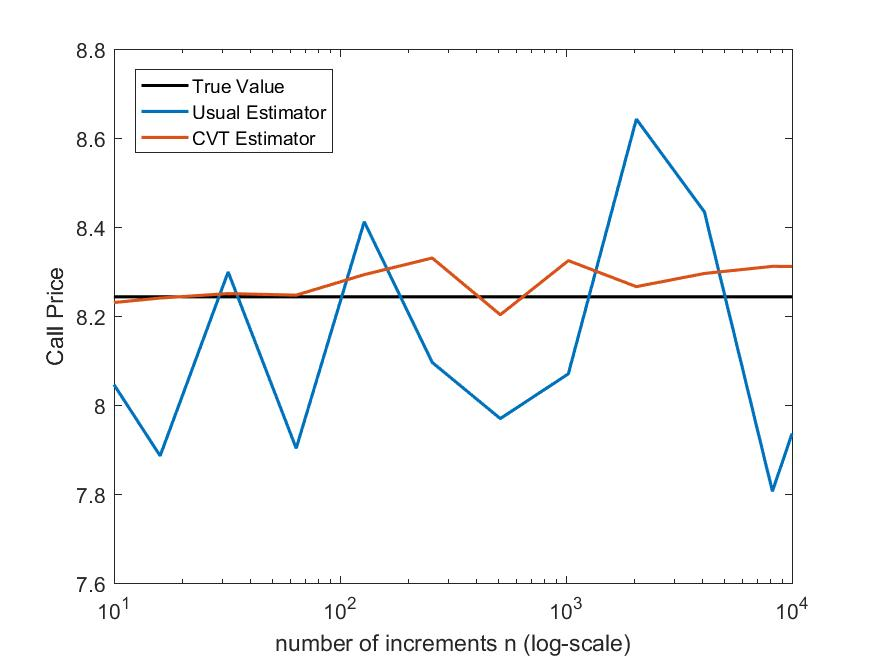
\includegraphics[width=8.5cm]{plot31.jpeg}
\end{subfigure}
\begin{subfigure}[c]{0.4\textwidth}
\caption*{N=10,000}
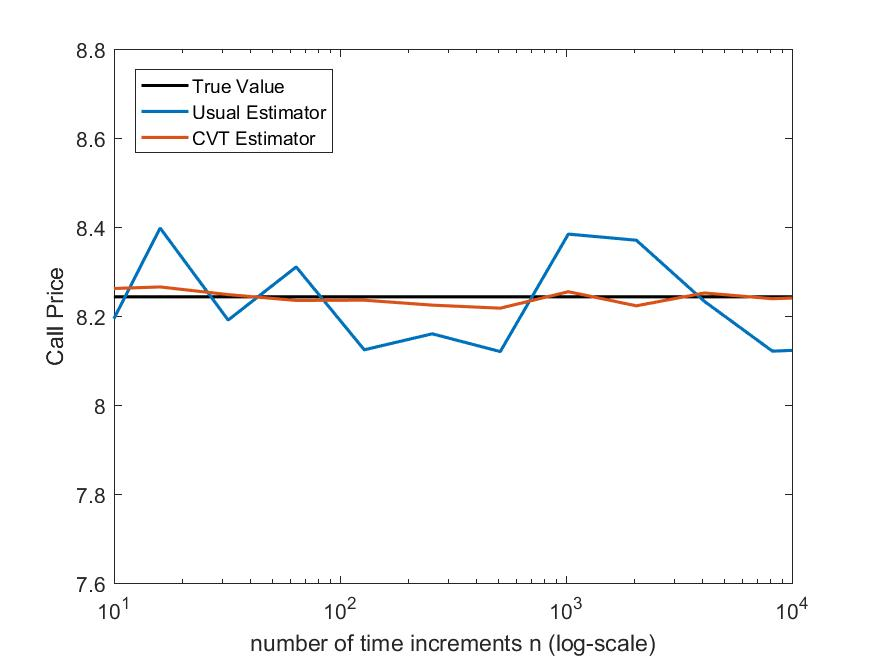
\includegraphics[width=8.5cm]{plot32.jpeg}
\end{subfigure}
\caption{Comparison of Time Increment Convergence for different N=1000 and N=10,000}
\label{plot31}
\end{figure}

\begin{figure}[!h]
\centering
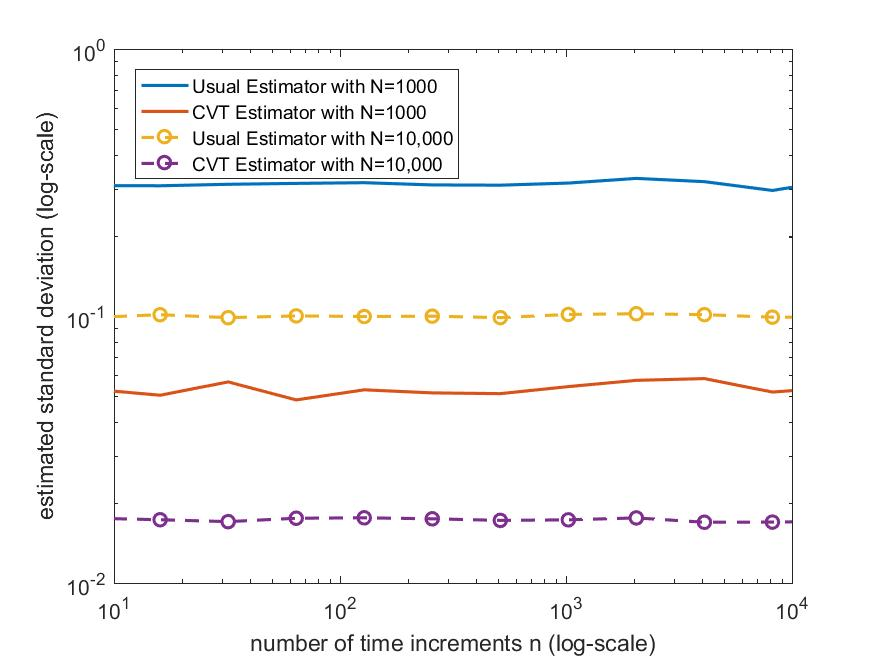
\includegraphics[width=11cm]{plot33.jpeg}
\caption{Time Increment Convergence - Estimated Standard Deviation}
\label{plot33}
\end{figure}

In figure \ref{plot31} it is  examined which effect an increase in time increments \textit{n} has on the accuracy for a fixed    \textit{N}=1000 and \textit{N}=10,000. What you can see is that the refinement of \textit{n} does not improve accuracy, either in the case of N=1000, nor in the case of N=10,000, independent of the choice of usual estimate or CVT. Volatility only reduces significantly for an increase in the number of simulated paths \textit{N}.

These findings are confirmed in illustration 9. Indeed, the estimated standard deviation stays constant in all four cases for an increase in \textit{n}. Hence an increase in \textit{n} does not influence accuracy or efficiency. This is not surprising because the CVT modification by its nature affects the sampling error, not the discretisation error. Furter examinations regarding time efficiency were therefore skipped.

\newpage
\subsection{Technical Implementation}
All associated computations of chapter 3 are splitted into two main scripts \textit{Problem2a.m} and \textit{Problem2b.m} where the main algorithms \textit{MC\_USUAL.m} for the usual estimator and \textit{MC\_CVT.m} for the CVT modification are called. 

As an input of the algorithms we used the given parameters, the discretisation steps \textit{nn} and the number of simulation paths \textit{NN}. Again, two pseudo-random numbers with a combined multiple recursive random number generator were generated with help of the specified \textit{Rand.Generator} and the \textit{randn} command.

What was noticeable is how these errors behaved. The errors marginally differed when calling them in the algorithm function itself compared if they are generated outside the function in the main script. It seems that \textit{MATLAB} does not only generate pseudo-random numbers specified by the initialization seed value but also on the location where these numbers were generated. Generating random numbers in the algorithm \textit{MC\_USUAL.m} hence slightly differed compared to the errors in the algorithm \textit{MC\_CVT.m} since they are not generated in the same location. Indeed, this would have an effect on comparability of the findings. Therefore we decided to generate the errors outside the algorithms in the main script and handle them as additional input parameters of the functions \textit{MC\_USUAL.m} and \textit{MC\_CVT.m}.

Both algorithms basically are constructed in the same manner as it was discussed in the theoretical framework of this chapter. The first part of \textit{Problem2a.m} consists of the proof that efficiency factor $\varrho$ holds as it was described in the theoretical part. By calling this subsection you can see that the estimated variances Var\_CVT and Var\_U are equal for a CVT run with N=1000 or a run with the usual estimator with \textit{N\_EF}=30491. 

The second part of the main script \textit{Problem2a.m} consists of the loops for increasing \textit{NN} and fixed \textit{nn}. The findings are saved in the output matrix \textit{SZ\_usual} and \textit{SZ\_CVT} for the usual and CVT case, respectively. The exact specification of each column can be found in the code. All these findings are plotted in the usual manner with help of the \textit{plot} or \textit{semilogx} commands. The time was again measured with the \textit{tic} and \textit{toc}commands and can differ depending on the system.

The main script \textit{Problem2b.m} is constructed in the same fashion but in that case we fixed \textit{NN} and looped over \textit{nn}. All findings again are saved in specified output vectors which are then plotted.

Note that the Monte Carlo approach can be relatively time consuming, so the number of simulations was set to a maximum of \textit{NN}=10,000 because it delivers precise results in a reasonable time. However, the program was written dynamically, so the parameter NN can be increased when running on more powerful system.

Again all computations were run on an Windows 10 64-bit operation system with an Intel(R) Core(TM) i7-5500U CPU 2.40 Ghz.
\newpage

\section{References}

Betkaoui, Brahim, David B. Thomas, and Wayne Luk. \textit{Comparing performance and energy efficiency of FPGAs and GPUs for high productivity computing.} Field-Programmable Technology (FPT), 2010 International Conference on IEEE, 2010.
\\

Brandimarte, Paolo. \textit{Numerical Methods in Finance and Economics. - A MATLAB- Based Introduction}, 2nd ed., John Wiley and Sons, Hoboken NJ, 2006.
\\

Glassermann, Paul. Monte Carlo Methods in Financial Engineering, Springer Verlag, New York 2003.
\\

Sch\"obel, Rainer and Jianwei Zhu. \textit{Stochastic Volatility With an Ornstein-Uhlenbeck Process: An Extension.} European Finance Review 3, 1999, 23 - 46.
\\
\end{document}
